\begin{appendices}


\renewcommand{\thechapter}{A}
\chapter{Figure}
\label{immagini}
In questa appendice si riportano le figure che si è preferito riportare separatamente rispetto al contenuto principale dell'elaborato di tesi.

\vfill
\pagebreak[4]

\section{Addestramento delle CNN mediante transfer learning e calcolo delle prestazioni}

\subsection{AlexNet}

\begin{figure}[h!]
  \centering
  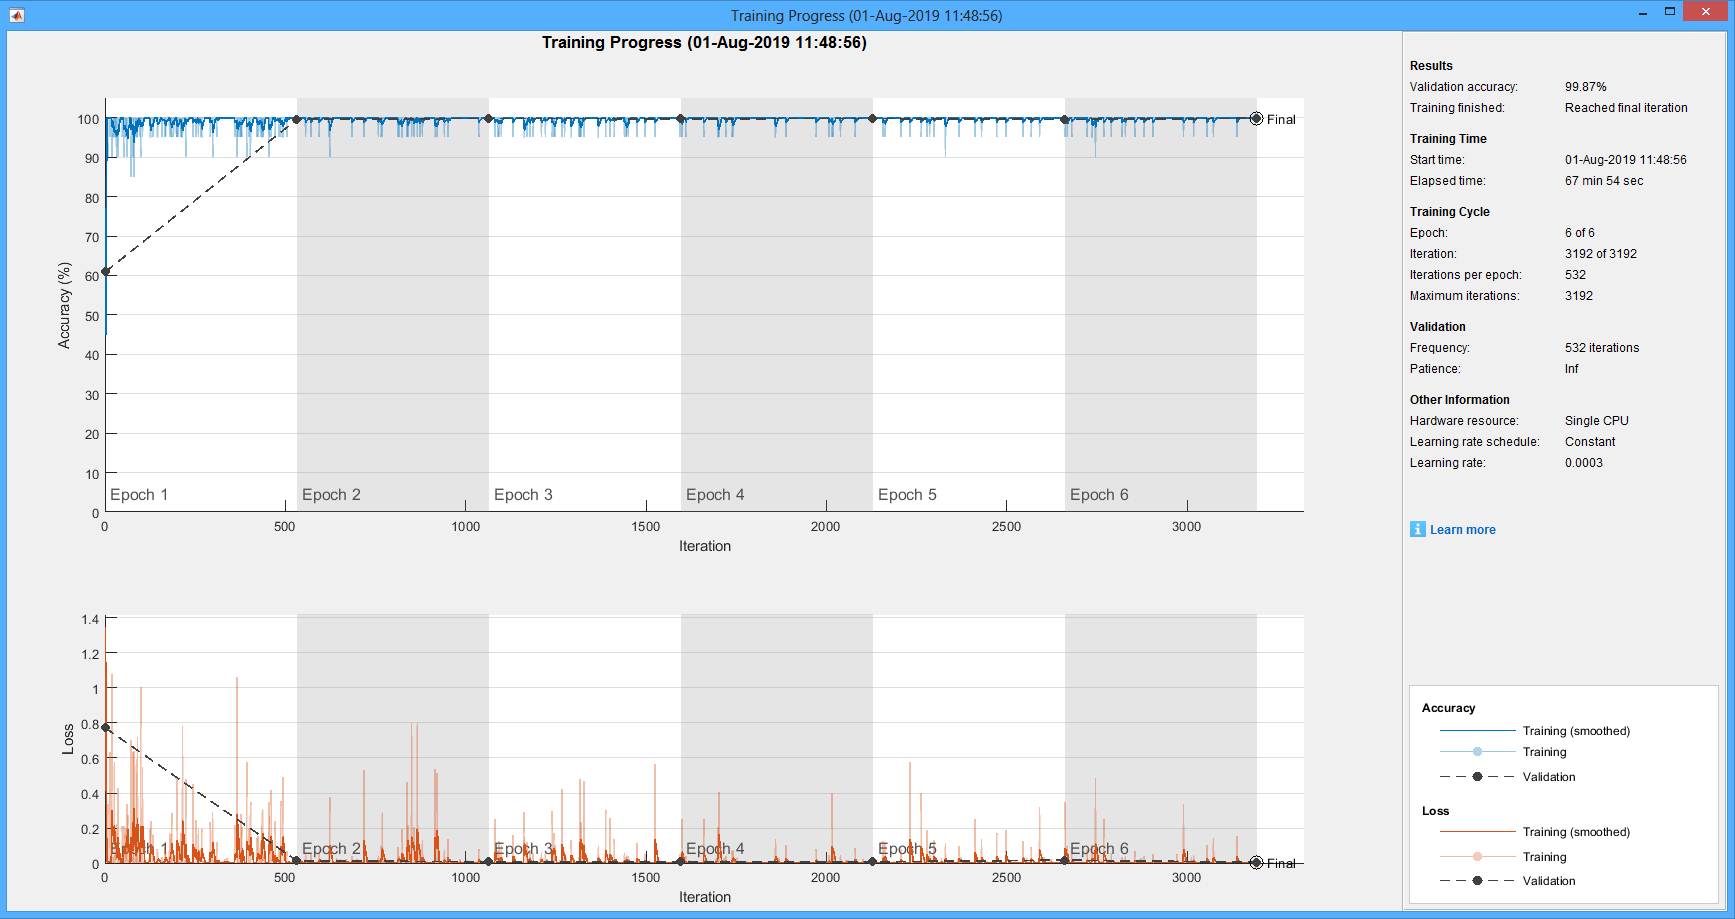
\includegraphics[width=\textwidth]{TrainingAlexNet.png}
  
  \caption{Grafico del ri-addestramento di AlexNet}

\end{figure}


\begin{figure}[h!]
  \centering
  \begin{subfigure}[b]{0.45\linewidth}
    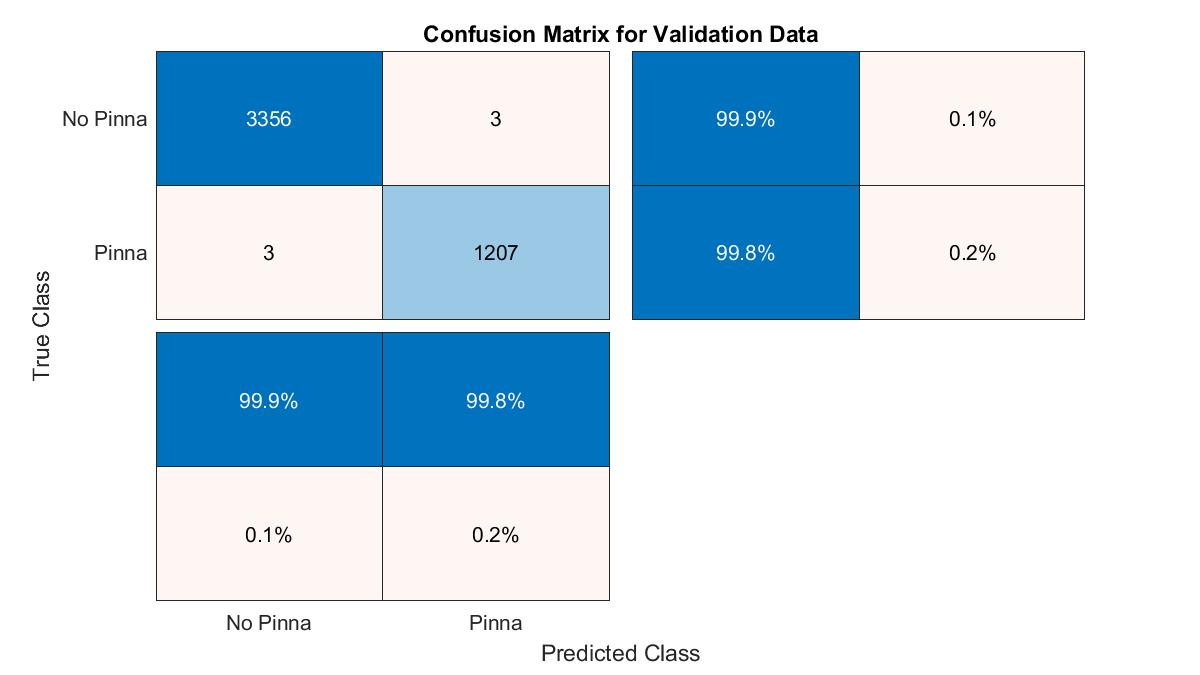
\includegraphics[width=\linewidth]{confMatAlexNet.jpg}
    \caption{}
  \end{subfigure}
  \begin{subfigure}[b]{0.45\linewidth}
    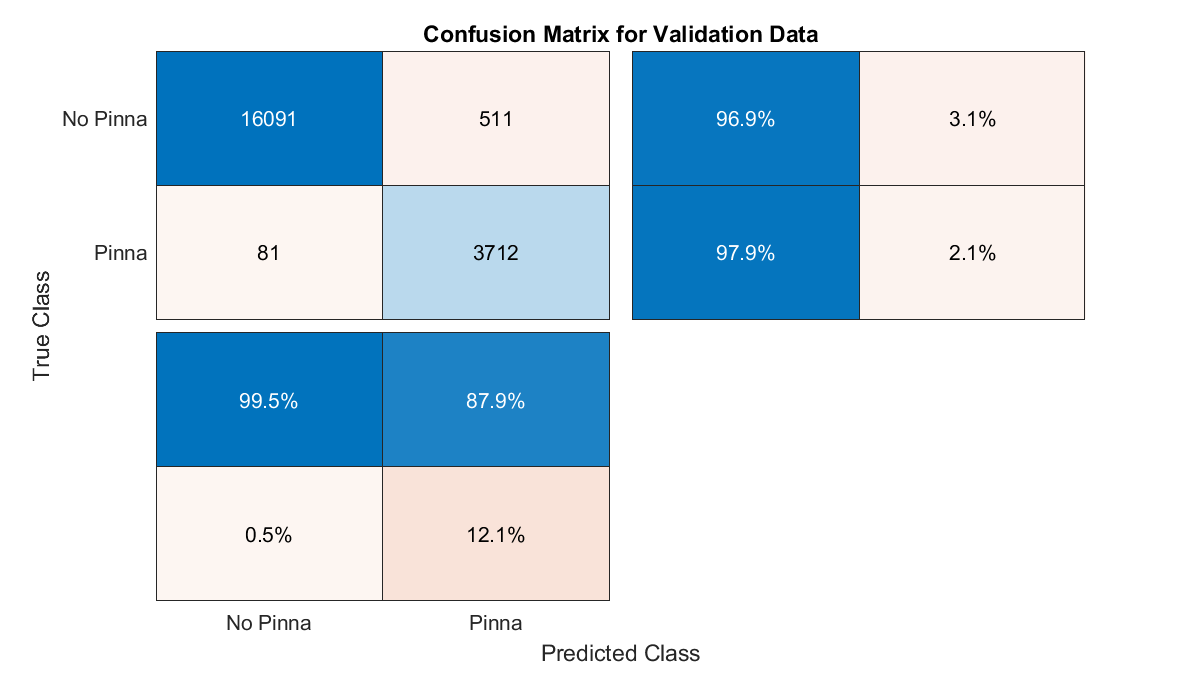
\includegraphics[width=\linewidth]{confMatAzzorrealexnet.png}
    \caption{}
  \end{subfigure}
  
  \caption{Matrice di confusione relativa all'impiego di AlexNet nella classificazione di (a) ritagli di Taranto, (b) ritagli delle Azzorre.}

\end{figure}

\vfill
\pagebreak[4]

\subsection{GoogLeNet}

\begin{figure}[h!]
  \centering
  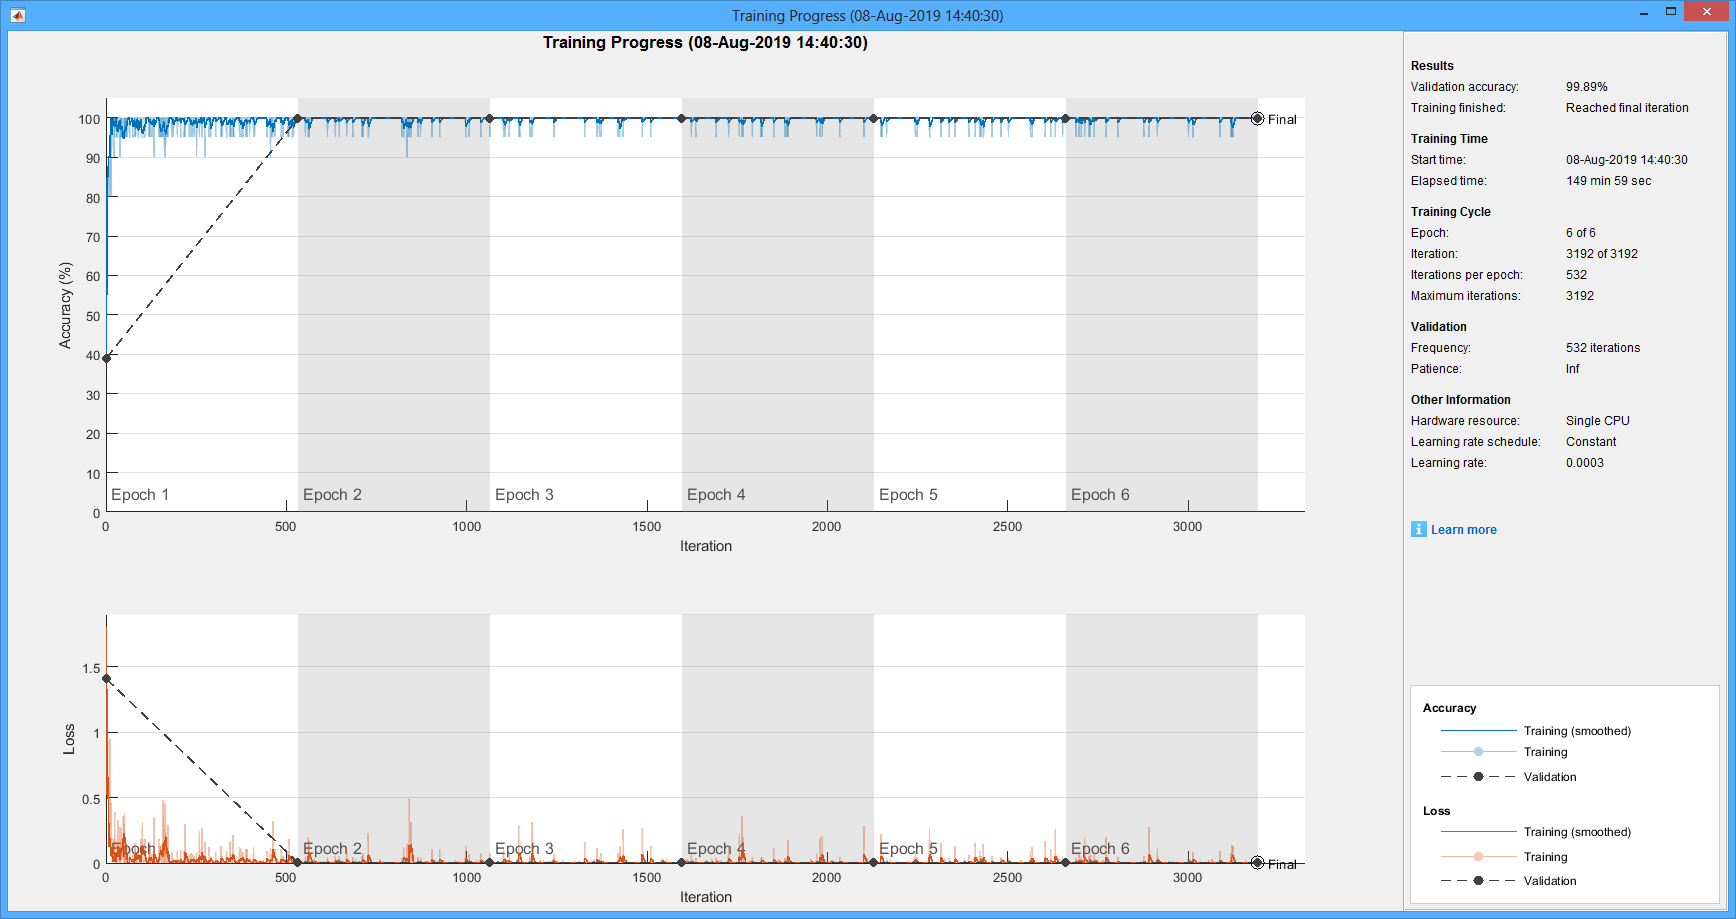
\includegraphics[width=\textwidth]{TrainingGoogLeNet.png}
  
  \caption{Grafico del ri-addestramento di GoogLeNet}

\end{figure}


\begin{figure}[h!]
  \centering
  \begin{subfigure}[b]{0.45\linewidth}
    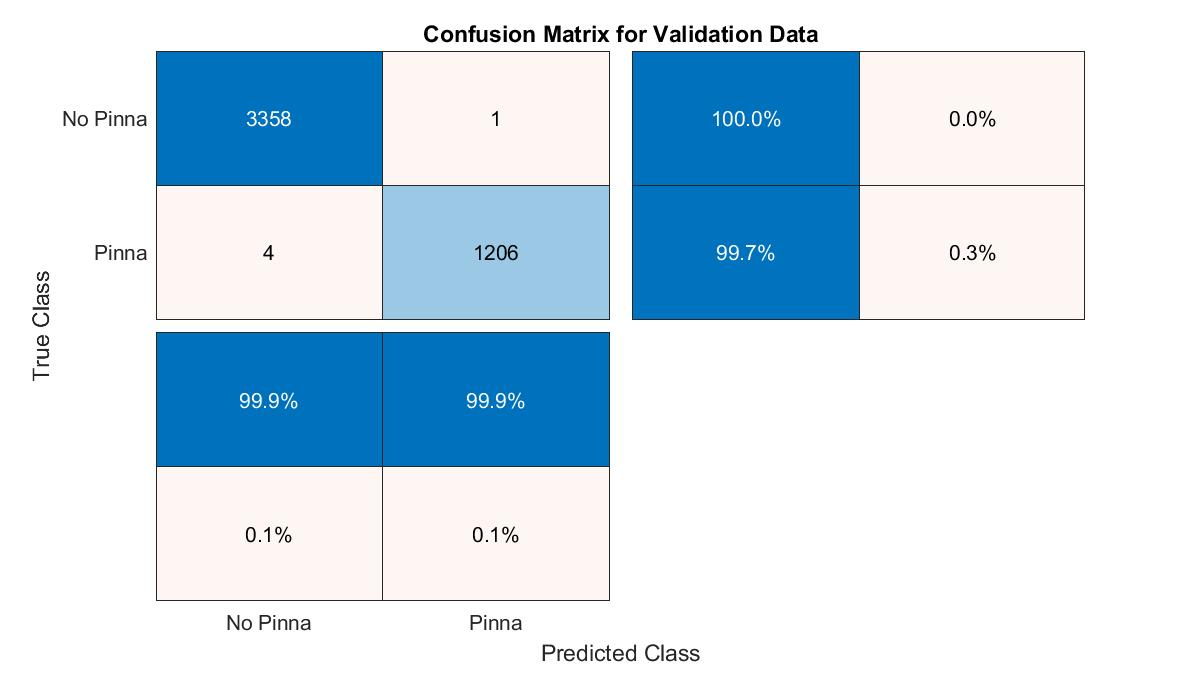
\includegraphics[width=\linewidth]{confMatGoogLeNet.jpg}
    \caption{}
  \end{subfigure}
  \begin{subfigure}[b]{0.45\linewidth}
    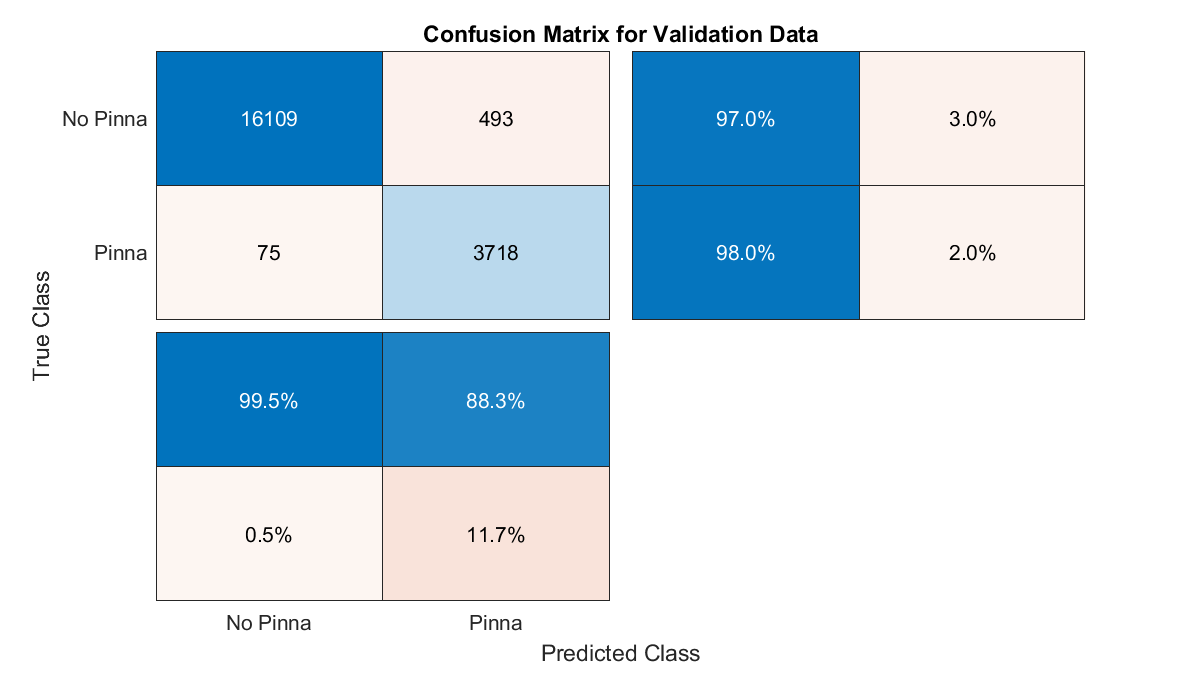
\includegraphics[width=\linewidth]{confMatAzzorregooglenet.png}
    \caption{}
  \end{subfigure}
  
  \caption{Matrice di confusione relativa all'impiego di GoogLeNet nella classificazione di (a) ritagli di Taranto, (b) ritagli delle Azzorre.}

\end{figure}

\vfill
\pagebreak[4]

\subsection{ResNet-18}

\begin{figure}[h]
  \centering
  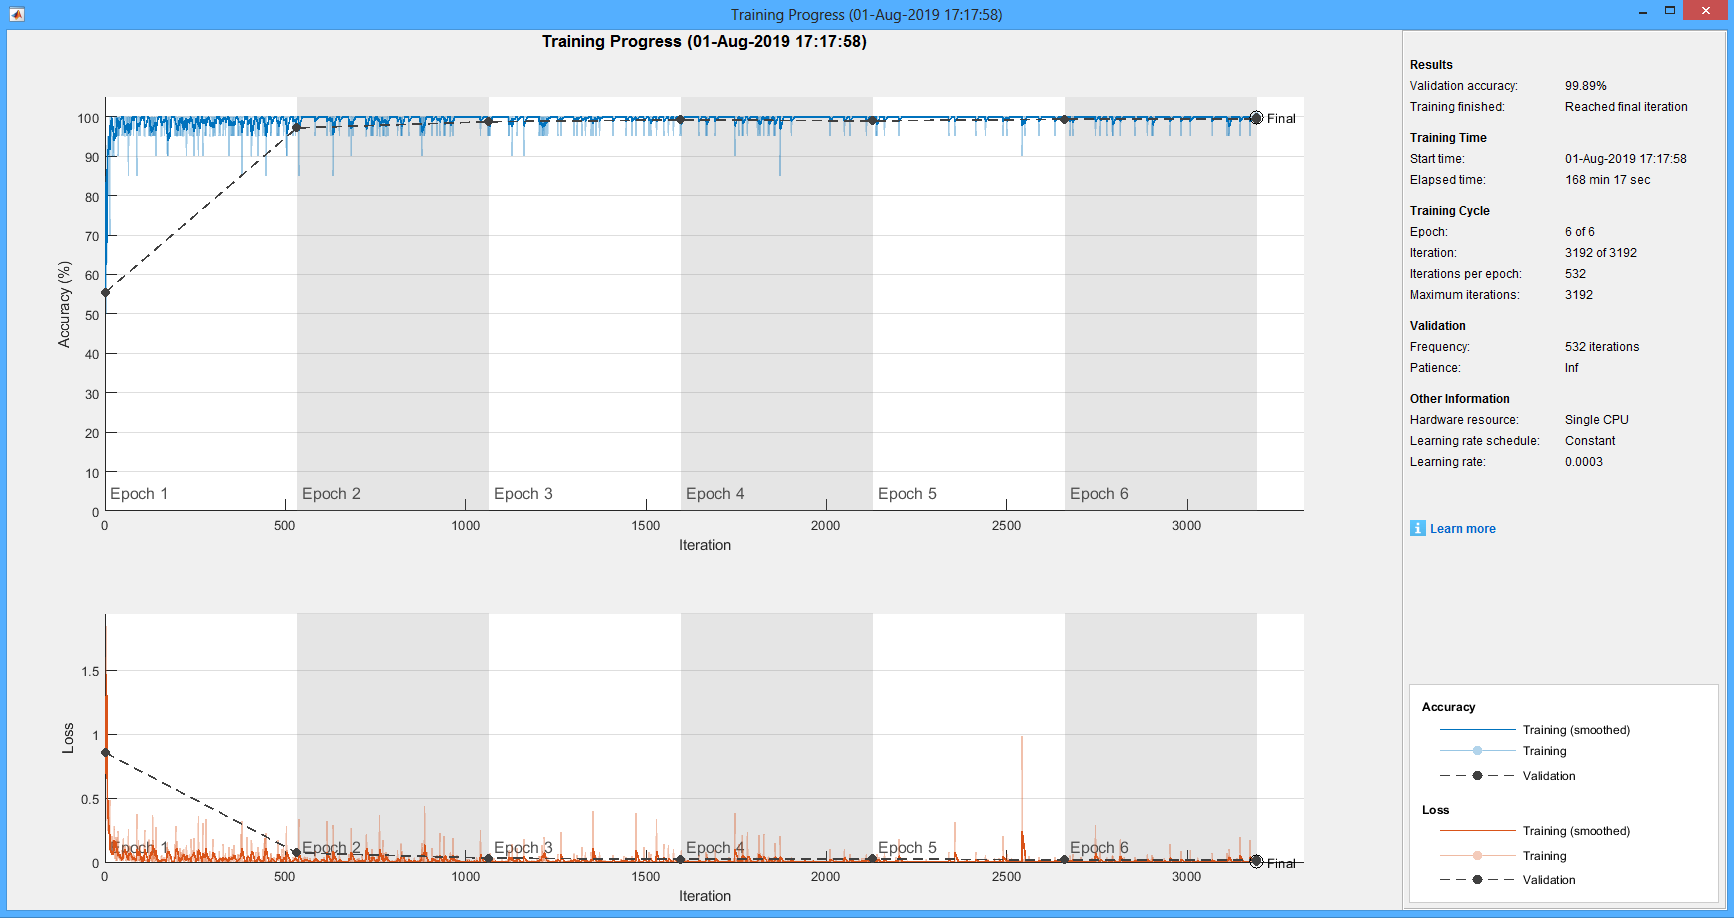
\includegraphics[width=\textwidth]{TrainingResNet18.png}
  
  \caption{Grafico del ri-addestramento di ResNet-18}

\end{figure}


\begin{figure}[h!]
  \centering
  \begin{subfigure}[b]{0.45\linewidth}
    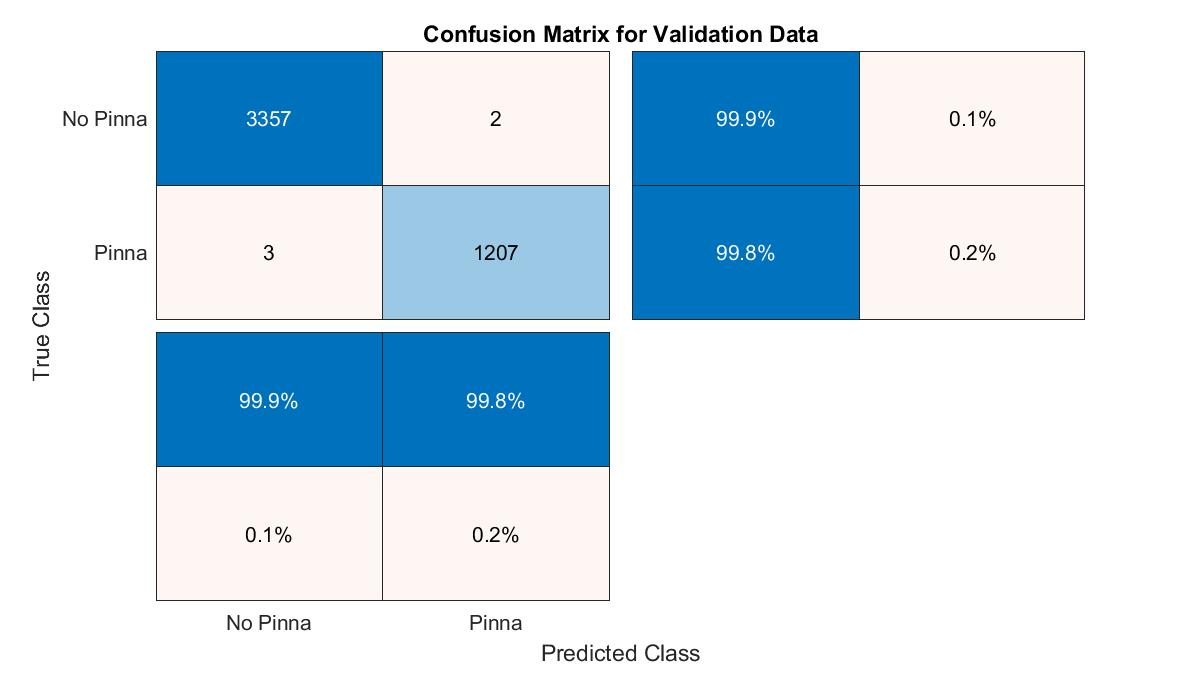
\includegraphics[width=\linewidth]{confMatResNet18.jpg}
    \caption{}
  \end{subfigure}
  \begin{subfigure}[b]{0.45\linewidth}
    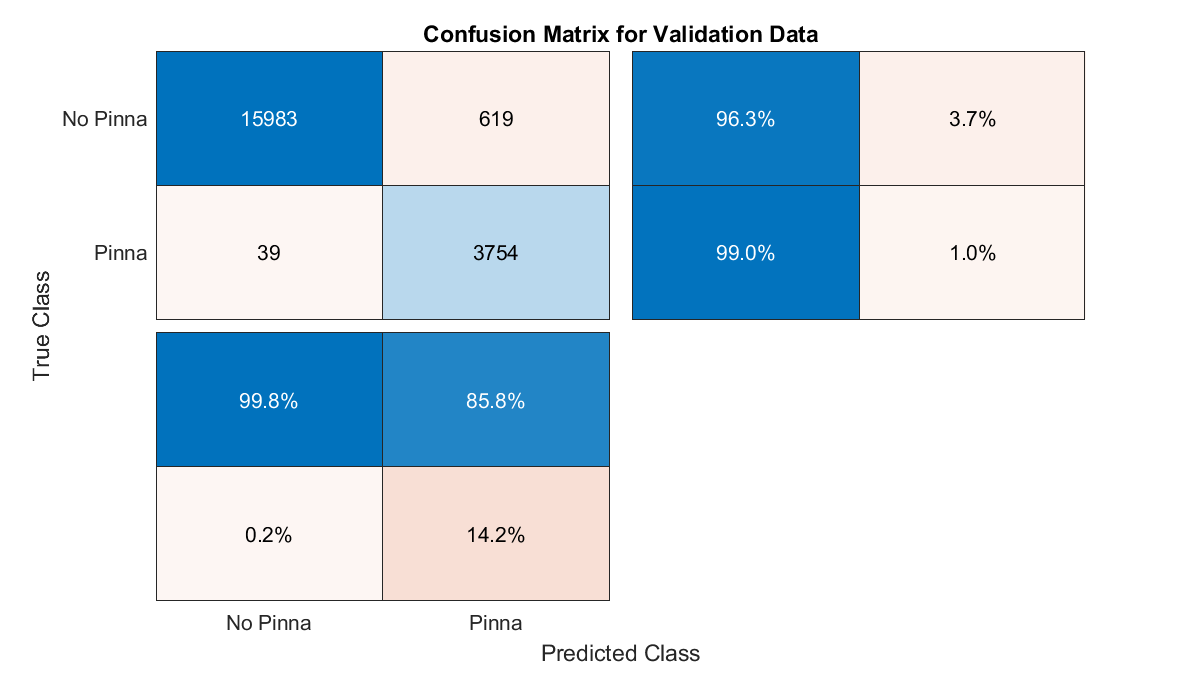
\includegraphics[width=\linewidth]{confMatAzzorreresnet18.png}
    \caption{}
  \end{subfigure}
  
  \caption{Matrice di confusione relativa all'impiego di ResNet-18 nella classificazione di (a) ritagli di Taranto, (b) ritagli delle Azzorre.}

\end{figure}

\vfill
\pagebreak[4]

\subsection{ResNet-50}

\begin{figure}[h]
  \centering
  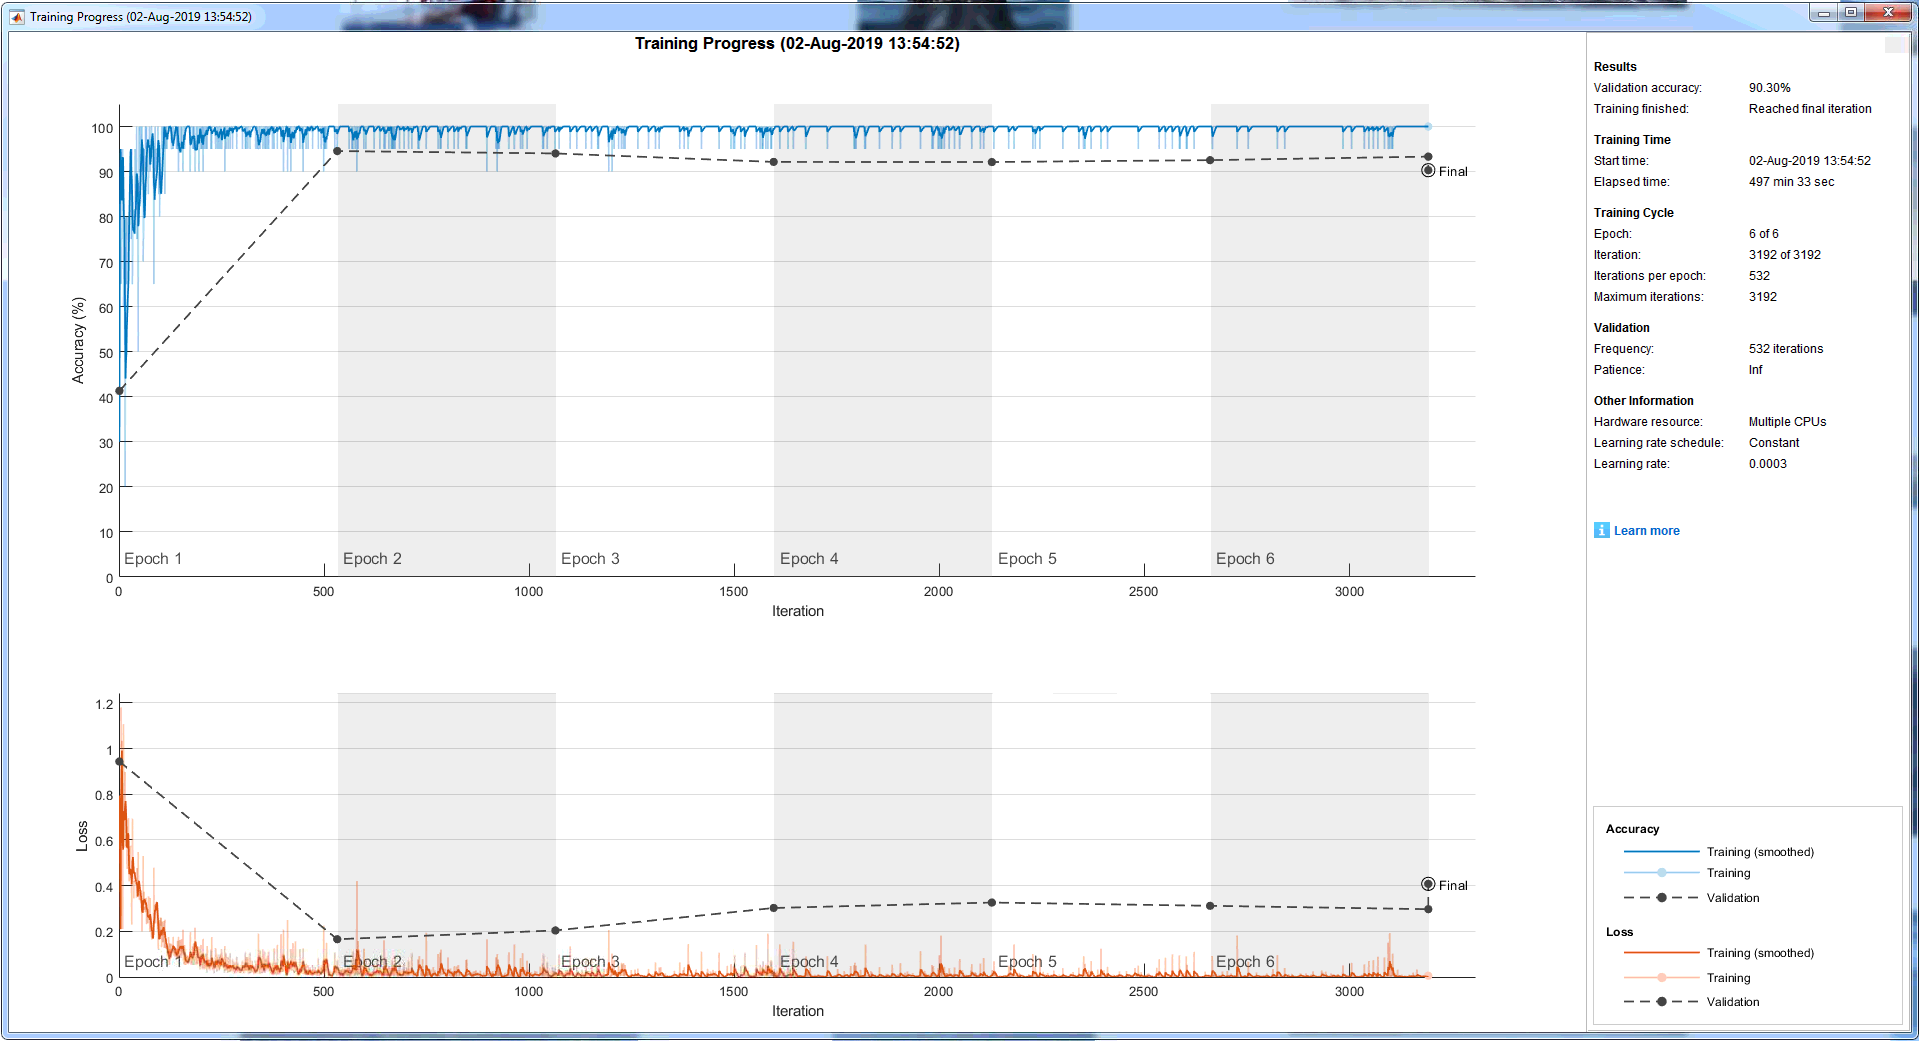
\includegraphics[width=\textwidth]{TrainingResNet50.png}
  
  \caption{Grafico del ri-addestramento di ResNet-50. Si noti che la \textit{training accuracy} è prossima al 100\% mentre la \textit{validation accuracy} si attesta al 90\%, chiaro sintomo di \textit{overfitting} al training set.}

\end{figure}


\begin{figure}[h!]
  \centering
  \begin{subfigure}[b]{0.45\linewidth}
    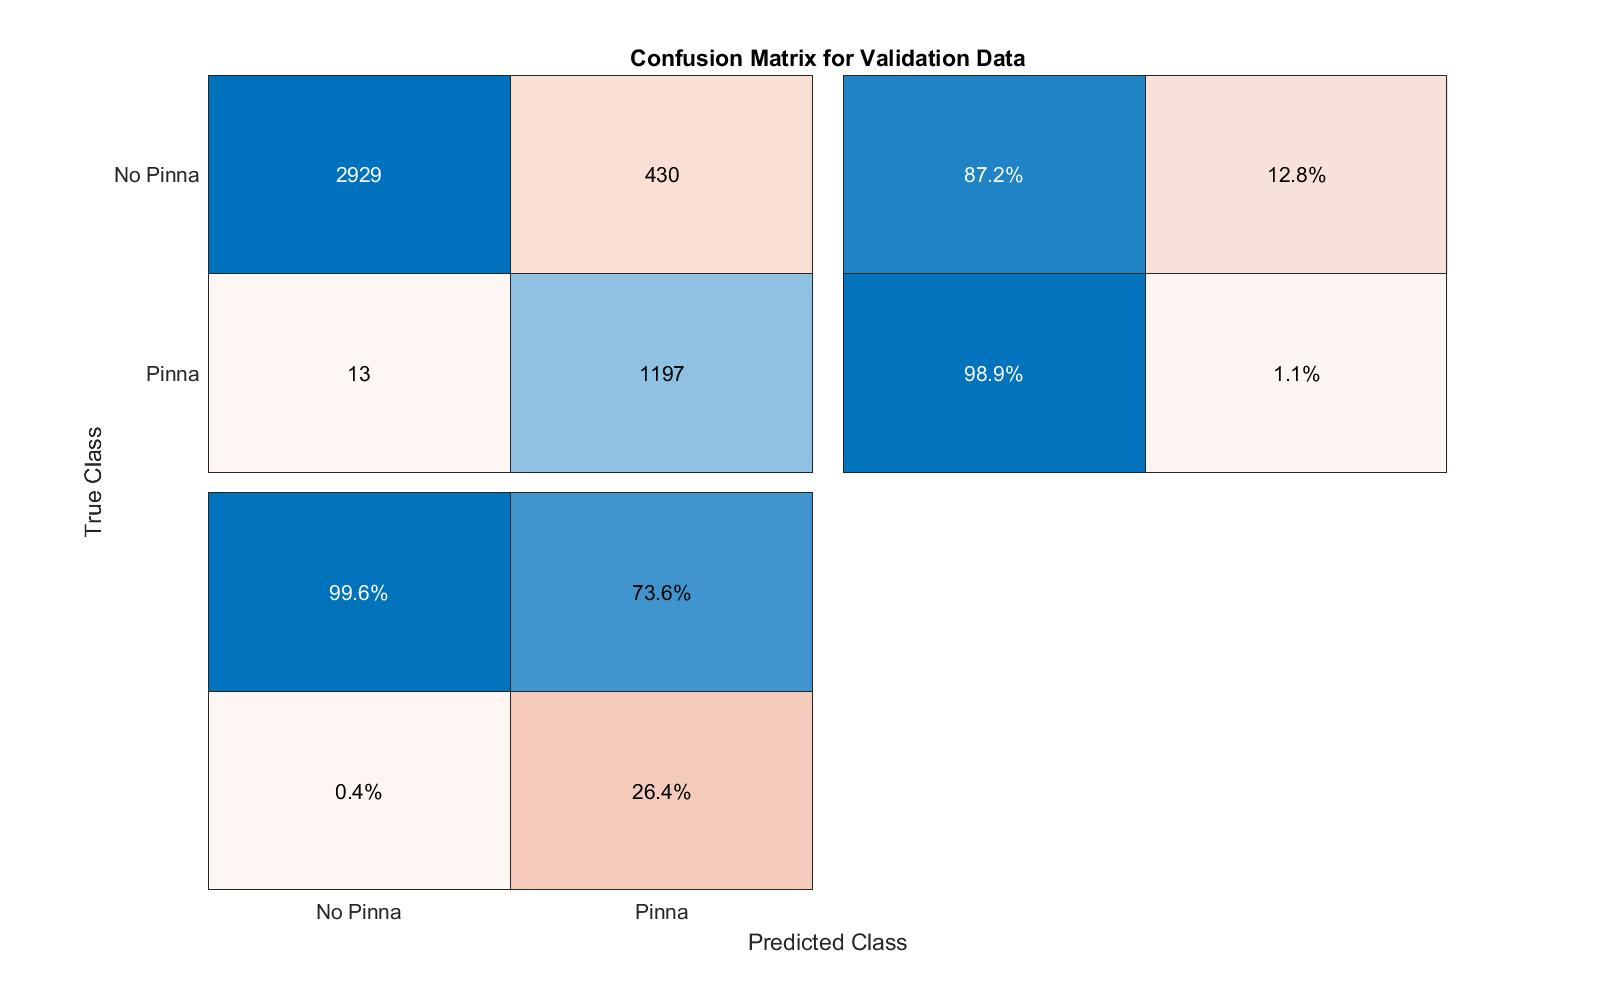
\includegraphics[width=\linewidth]{confMatResNet50.jpg}
    \caption{}
  \end{subfigure}
  \begin{subfigure}[b]{0.45\linewidth}
    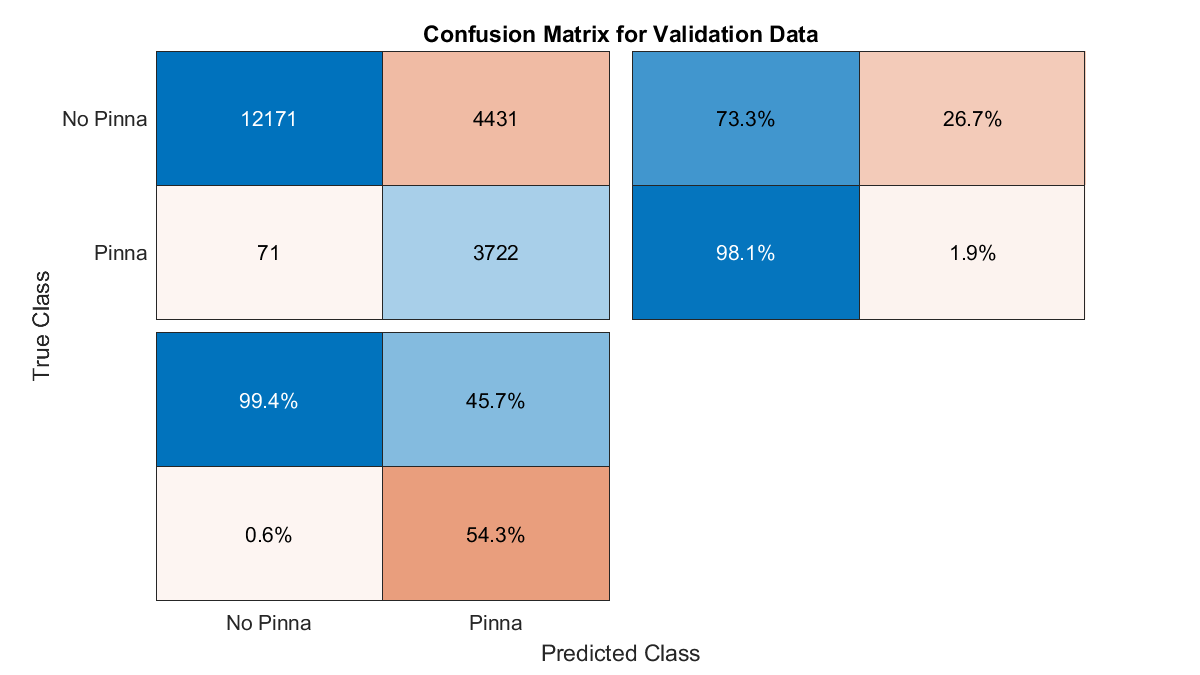
\includegraphics[width=\linewidth]{confMatAzzorreresnet50.png}
    \caption{}
  \end{subfigure}
  
  \caption{Matrice di confusione relativa all'impiego di ResNet-50 nella classificazione di (a) ritagli di Taranto, (b) ritagli delle Azzorre. Si noti l'eccessivo numero di falsi positivi.}

\end{figure}

\vfill
\pagebreak[4]

\subsection{Ensemble (Alexnet + GoogLeNet + ResNet-18)}

\begin{figure}[h!]
  \centering
  \begin{subfigure}[b]{0.45\linewidth}
    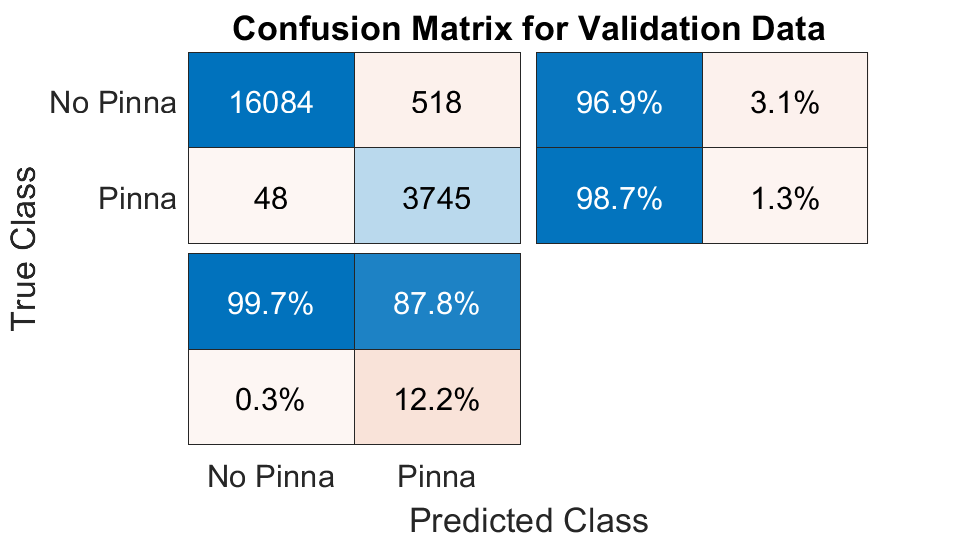
\includegraphics[width=\linewidth]{confMatAzzorreSMV.png}
    \caption{}
  \end{subfigure}
  \begin{subfigure}[b]{0.45\linewidth}
    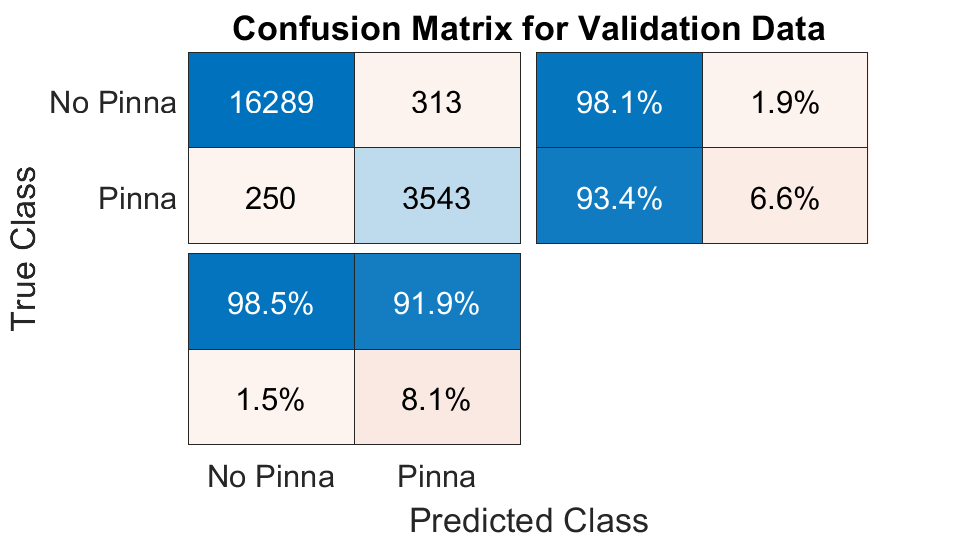
\includegraphics[width=\linewidth]{confMatAzzorreHMVT.png}
    \caption{}
  \end{subfigure}
  
  \caption{Matrice di confusione relativa all'impiego dell'ensemble di CNN ri-addestrate nella classificazione dei ritagli di Taranto, con schema di consenso (a) \textit{soft major voting}, (b) \textit{hard major voting} con soglia sulla probabilità media della classe 'Pinna'}

\end{figure}


\end{appendices}